%==================================================================================================
%   LUKES THESIS TEMPLATE 1.2
%   -------------------------
%   This template is based upon the offcial IMM PhD Thesis template, it is enhanced with a number
%   of new features and a number of errors have fixed. This template is intended to be complied to
%   PDF using PDFLATEX and is tested using the MiKTeX 2.9 LaTeX distribution.
%   It is based on the official DTU-IMM Thesis template by Finn Kuno Christensen in 2009.
%   Small bugfixes by Kasper Laursen in 2012 and 2013.
%   Small updates by Finn Kuno Christensen/Henning Christiansen in 2015.
%   -------------------------
%   Last Updated: 2015-01-08
%==================================================================================================
%
%==================================================================================================
% DOCUMENT SETUP
%==================================================================================================
\documentclass[10pt,twoside]{book}                  %Official DTU-IMM Thesis document setup
%
%Set to 'print' for printed version, use 'net' for online version
\def\thesisversion{print}
%
%==================================================================================================
% PACKAGES
%==================================================================================================
\usepackage{LukeThesis}                             %Import Thesis base style
\usepackage{booktabs}
\usepackage{tabularx}
\usepackage{float}
\usepackage{listings}
\usepackage{xcolor}


%input{PhDMacros}                                   %Thesis specific macros
%
%==================================================================================================
% THESIS PROPERTIES (Modifiy these fields with your details)
%==================================================================================================
\def\thesisauthor{Jens-Christian Finnerup}                     %Author
\def\thesistitle{Enabling Multirotors to Perform Construction Tasks Using Swarm Algorithms}               %Title
\def\thesishandin{01-August}                       %Submission date (Day-Month}
\def\thesisdegree{MSc}                              %Degree ('B.Eng', 'B.Sc.', 'M.Sc.' or 'PhD')
\def\thesisyear{2016}                               %Submission year
\def\thesisnumber{????}                             %DTU-IMM Serial number (do not include year)
\def\thesisISSN{0000-0000}                          %ISSN number
\def\thesiskeywords{Swarm Robotics, Drones, Construction, Formation Flight}  %PDF keywords
\derivethesisprops                                  %Derive dependent properties
%
%==================================================================================================
% SECTION NUMBERING SETUP
%==================================================================================================
\setcounter{tocdepth}{2}                            %2 adds sections up to subsections
\setcounter{secnumdepth}{3}                         %Subsubsections get a number when this is 3
%
%==================================================================================================
% THESIS STRUCTURE  (Modifiy to include more chapters etc)
%==================================================================================================
\begin{document}
%------------------------
%Pre-frontmatter material
%------------------------
\prefrontmatter
%--------------------
%Frontmatter material
%--------------------
\frontmatter
\pagenumbering{roman}                               %Set frontmatter numbering style
\input{Chapters/summaryUK}                                   %English summary of Thesis
\markboth{}{}                                       %Set headings (left)(right)
\input{Chapters/summaryDK}                                   %Danish summary of Thesis
\markboth{}{}                                       %Set headings (left)(right)
\input{Chapters/preface}                                     %Preface
\markboth{}{}                                       %Set headings (left)(right)
\input{Chapters/acknowledgements}                            %Acknowledgements
\markboth{}{}                                       %Set headings (left)(right)
%------------------
% Table of contents
%------------------
\newpage\mbox{}\newpage
\chaptermark{Contents}
\pdfbookmark{\contentsname}{toc}
\renewcommand{\sectionmark}[1]{\markright{#1}}
\sectionmark{Contents}
\addtolength{\parskip}{-\baselineskip}
\tableofcontents
\addtolength{\parskip}{\baselineskip}
\renewcommand{\sectionmark}[1]{\markright{\thesection\ #1}}
%-------------
% Main content
%-------------
\mainmatter
\include{Chapters/introduction} 

\chapter{Methodology}
In order to evaluate the different control algorithms and their performance, the approach towards designing and testing the algorithms must be systematic and concise. 
The different subproblems specified in \ref{intro:sub_problems}, can be said to either relate to either the simulation design or the algorithm design. As such, for the purpose of this thesis, a different approach will be used when dealing with constructing the simulation and when designing and testing the control algorithms. In this chapter, I will outline these approaches and the methodology used. The first three sections of this chapter will deal with the simulation methodology, whereas the latter three will deal with the implementation and testing of the control algorithms. 

\section{Control Problem}
The main research problem os this thesis involves building and evaluating different control algorithms, and as such each algorithm must be subject to the same evaluation technique.
This evaluation technique will throughout the thesis be referenced to as the \textit{Control Problem}, and the purpose of the agents will be so solve this problem collectively. 
As such the problem chosen must be the same problem throughout every simulation and independent of the control algorithms themselves. The problem must also be able to be solved collectively, by multiple agents at the same time, while still posing enough challenges to properly test the control algorithms. Posing dangers to the agents, such as the risk of collision. 

This control problem will exist within the simulation as a physical task that the agents have to carry out. Chapter \ref{sec:control_problem} will outline the concrete control problem used, as well a discussion on the specific control problem's advantages and limitations. 

\section{Simulation Construction}
The control problem and the simulation are mutually dependent, as the problem has to able to exist and be solvable within the simulation. As such the simulation has to be designed with the control problem in mind, but the control problem also has to be made with the limitations of the simulation taken into account. The simulation aspect is crucial to the validity of the results expressed in this thesis. For the purpose of solving the problems outlined in this thesis, the simulation will be a virtual environment, in which drones can be deployed. The drones will have to be subject to the same physical laws, as they would in real life such that the findings and test results can by applied to issues and control techniques in the real world.

In order to reduce complexity of the simulation, some physical laws are not taken into account when designing the simulation. This is done based on assumptions on which laws influence the results. An outline of the simulation design, can be found in Chapter \ref{chap:simulation}. 

\section{Validation}
Validation is a method to ensure that the simulation is mimicking real life physics and not simply animating the desired behavior of the drones. The validation will be carried out iteratively along with the construction of the simulation, to monitor the progress of the simulation construction, and act as a sort of checklist to the accuracy and capabilities of the simulation. The validation phase consists of multiple validation tests, meant to test if the simulation actually simulates the physical mechanics required. These mechanics can range from gravitational pull to accurate impulse and mass on the bodies in the simulation. The validation tests will when range from checking the accurate acceleration of drones in free fall etc. These validation tests are also important because the simulator must have the predictable behavior across many scenarios, such that they can be compatible. The validation tests will be discussed and outlined in Section \ref{sec:validation}

\section{Test Metrics}
Up until now this chapter on methodology has been focused on systematically creating and validating the simulation platform. The following part will be covering my approach to creating and testing the control algorithms. 

The comparison of the algorithms tested within this thesis, will be done based on their ability to solve the Control Problem. However the control problem must be designed in such a way, that it can be solved in to various degrees. To measure how well the control problem is solved, some metrics must be chosen so that they represent the challenges of the control problem. I.e. if the control problem challenges the agents in collision avoidance, a test metric could be the each agents distance the all other agents over time. The metrics chosen will be covered in Chapter \ref{chap:simulation} and will in part be based challenges of swarm robotics covered in \texttt{Multi-robot navigation in formation via sequential convex programming} \cite{alonso-mora_multi-robot_2015}.

\section{Experimentation}

\section{Optimization}



\begin{figure}[h!]
  \centering
  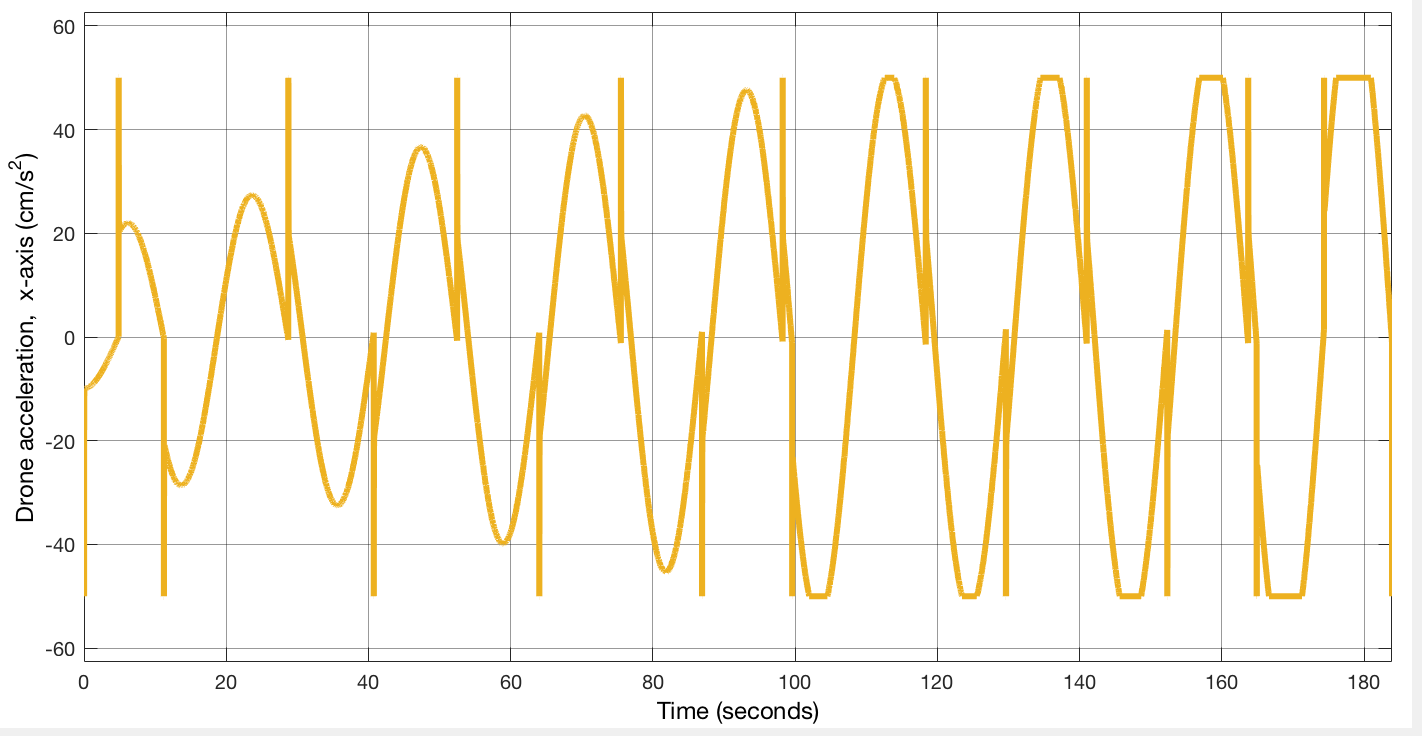
\includegraphics[width=.8\columnwidth]{figures/SA_accel_with_no_vel_limit.png}
  \caption{Acceleration of agent - without velocity limit}
  \label{fig:sa_accel_no_vel_adj}
\end{figure}






 
\include{Chapters/simulation}

\chapter{Swarm Logic \& Swarm Algorithms}
\label{chap:swarm}

\section{Multi-body vs. Multi-agent path planning}
%master slave principle, single point of failure, etc.

                                 %Chapter 1

\chapter{3-Dimensional Stigmergy}
\label{chap:stigmergy}

This chapter will outline the implementation attempt of the a stigmergy control algorithm, as well as some of the theory behind pheromone controlled agents. 
 
\section{Digital Markers (Pheromones)}
In the world of biology, stigmergy refers to using pheromones as a means of communication between agents. Originally described by (Grasse 1959)\cite{holland_stigmergy_1999}  as the way that termites or ant colonies maintain efficiency and overall planning when building hives. Pheromones are put in place by the agents as a marker to reinforce the behavior of other agent. Pheromones can be weakened over time or amplified by other agents passing over them, and as such the influence of the pheromones on the environment are increased.

Several implementations of algorithms using stigmergy have been attempted in a 2-dimensional space, however my literature research found limited evidence of attempts of using stigmergy in 3 dimensions to control flying vehicles. 

\section{Implementation}
\label{stigmergy:impl}

\subsection{Assumptions}
The implementation of this stigmergy based algorithm, operates under the assumption that an agent can identify an object of interest when the object is within a certain distance from the agent. This is necessary for the stigmergy algorithm to work as a complete solution to navigating the agents, as the pheromones only serve to guide the agents in specific directions. As such, without the agents' ability to identify objects of interest, they would simply move in a more efficient manner, but without performing the desired actions when arriving at their desired location. As such, it is assumed that the agents know to pick up a block or put it down, when they find themselves at the location where this is supposed to happen. 

This removes an element of complexity from the swarm algorithm, but is considered a fair assumption. It is therefore also assumed that this can be physically implemented with current sensor technology and object recognition, without negatively affecting the behavior of the stigmergy algorithm. 

\subsection{Specifications}
There are multiple variables to consider when implementing a pheromone based control algorithm. As the pheromones only represent a common set of information shared by all agents, in an otherwise decentralized environment, it is important to consider how this information is interpreted by the agents.  
The first implementation attempt was done with the parameters identified in Table \ref{tab:vars1}

\begin{table}[H]
\centering
\label{tab:vars1}
\begin{tabularx}{0.6\textwidth}{ll}
\toprule
\textbf{Variables}     & \textbf{Value}  \\ \hline
Pheromone grid size    & $30 \times 10 \times 10$ \\ \hline
Pheromone fatigue      & $0/s$               \\
Number of pheromone grids      & $1/s$               \\
Constant pheromone  & $0.2$             \\
Triggered pheromone & $1$               \\
View radius of agent   & $2 \times agent-radius$ \\
Agent states           & $4$               \\ \hline
\end{tabularx}
\caption{Specifications of 3D Stigmergy implementation}
\end{table}

\begin{itemize}
\item{The \textbf{Pheromone grid} is an empty $30x10x10$ matrix, containing only zeroes as the initial value. This is how the pheromones will be represented in 3 dimensions. The size and shape of this array is the same as the simulation environment, and when a pheromone is placed in space, the value of the pheromone will change from zero to the desired pheromone value}
\item{\textbf{Pheromone fatigue} refers to the decrease in all pheromones over time. This is used to determine how long a pheromone can remain \textit{unused} before it fades and no longer has any effect on the behavior of the agents. The initial implementation was done with zero fatigue to observe the effect of having permanent pheromones}
\item{\textbf{Constant pheromone} refers to the value that will be placed in the pheromone grid, just by an agent passing over it. \textbf{Triggered pheromone} will be the higher of a pheromone that the agent places in the grid, after having found an object of interest. Going back to the control problem, this can either be a block to be placed in the construction, or the area in which the block is supposed to be placed}
\item{\textbf{View radius of agent} works on the assumptions , that any agent is able to identify an object of interest, as long as it is within a given radius}
\item{\textbf{Agent states} is the number of states that an agent can be in, which in the case of the first implementation attempt is chosen to be four}
\item{\textbf{Number of pheromone grids} translates into the number of different kinds of pheromones }
\end{itemize}

\subsection{State machine diagram}
Figure \ref{fig:state_machine} shows the state machine diagram of the agents as implemented in this stigmergy algorithm. The goal of the agent is (as described in the control problem section) to find and collect blocks, and place them in the desired (yet simple) construction. As the figure shows, the agent has 4 states, where the most important part of the figure, is the transition from the first to the second, and the third to the fourth state. In these transition the agent uses the pheromone grid to choose an area to search for either a block or a goal in. Goals refer to the desired position of a block.

% Agent and simulation
\begin{figure}[H]
	\centering
	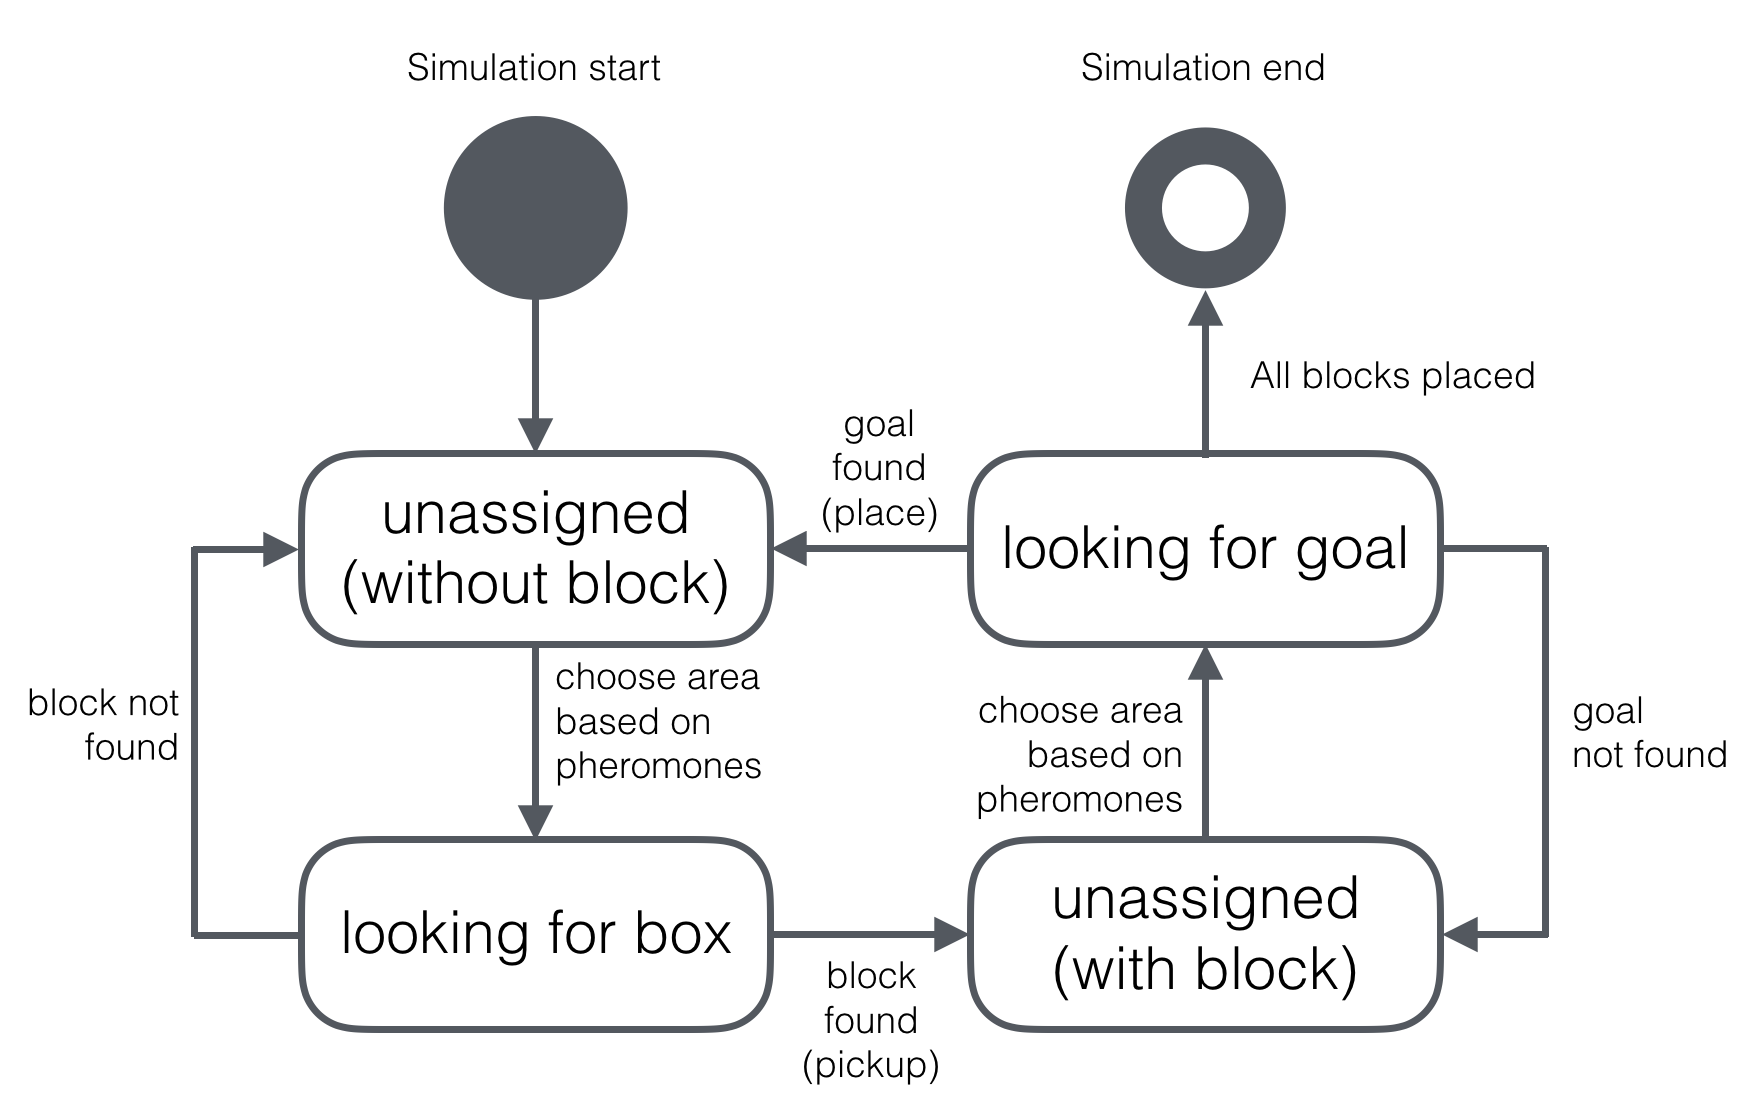
\includegraphics[width=1\columnwidth]{figures/state_machine}
  	\caption{\label{fig:state_machine}State machine diagram for an agent (including simulation start/finish)}
\end{figure}


\subsection{Development of pheromones}
The pheromones in the pheromone grid, are initially all given the value of zero. What this practically means is that there are not pheromones present in the simulation environment initially. In order for the pheromones to develop over time and affect the behavior of the agents, the agents themselves need to place them. This requires a set of general conditions under which the pheromones should be placed, which are outlined in Table \ref{tab:pheromones}.

\begin{table}[H]
\centering
\label{tab:pheromones}
\begin{tabularx}{1\textwidth}{llr}
\toprule
\textbf{Situation}     & \textbf{Action}   & \textbf{Condition}  \\ \hline
Block found & place pheromone with value 1 & none \\
Goal found & place pheromone with value -1 & none \\
At any time & place pheromone with value 0.2 & pheromone < 0.2 \\ \hline
\end{tabularx}
\caption{Rules for pheromone placement}
\end{table}

The negative pheromone value of the goal, represents a practical way of distinguishing pheromones that lead to the goals, from the pheromones that lead to blocks. This builds on an assumption of 

\subsection{Reacting to Pheromones}
When the pheromones have started developing in the environment, the agents need to react to them for the pheromones to have any influence. As previously mentioned, this happens after state 1 and 3, which is shown in Figure \ref{fig:state_machine}. 

The pheromones will influence the search of the agents and different strategies can be used to determine in what way. In the bullet points below i have listed some considerations that arose, from implementing effect of pheromones on the agents.

\begin{itemize}
\item{\textbf{Limit search space} - One way that the agents can react to pheromones, is to only move along paths that have already been marked with a pheromone value. This is essentially still a random search in space, but within a more limited scope, which suggests that it could be faster than without pheromones}
\item{\textbf{Strongest pheromone} - Instead of performing a random search throughout the environment, another simply way to use pheromones as guides is to go for the strongest pheromone (highest or lowest value depending on state). If the strongest pheromones are placed at the blocks and the goals over time, then these would be efficient to find if the agents are looking for the strongest pheromone}
\item{\textbf{Distance effects} - A slightly more complex way of using the pheromones to navigate, is to perform a distance calculation to the pheromones in the grid, and make the pheromones closest appear stronger than the ones further away}
\end{itemize}

Before any pheromone is placed in the grid, the search strategy for all agents is \textbf{random search} through out the level. The concrete implementation of the stigmergy algorithm, uses the a mix of all three strategies mentioned above, when a pheromone is present. 

The actual Matlab code of the implementation can be found in Appendix A.


\section{Testing}
\label{chap:stigmergy_test}

The following section includes the testing of the algorithm described above, and an evaluation of the test metrics outlined previously in Section \ref{sec:test_metrics}
\subsection{Pheromone grid}

After running the algorithm on the agents, the agents where able to complete the control problem successfully. The pheromone grid continuously evolved throughout the simulation, and after execution, the pheromone grid had the values which are shown in Figure \ref{fig:phero_post}.

% Pheromones
\begin{figure}[H]
	\centering
	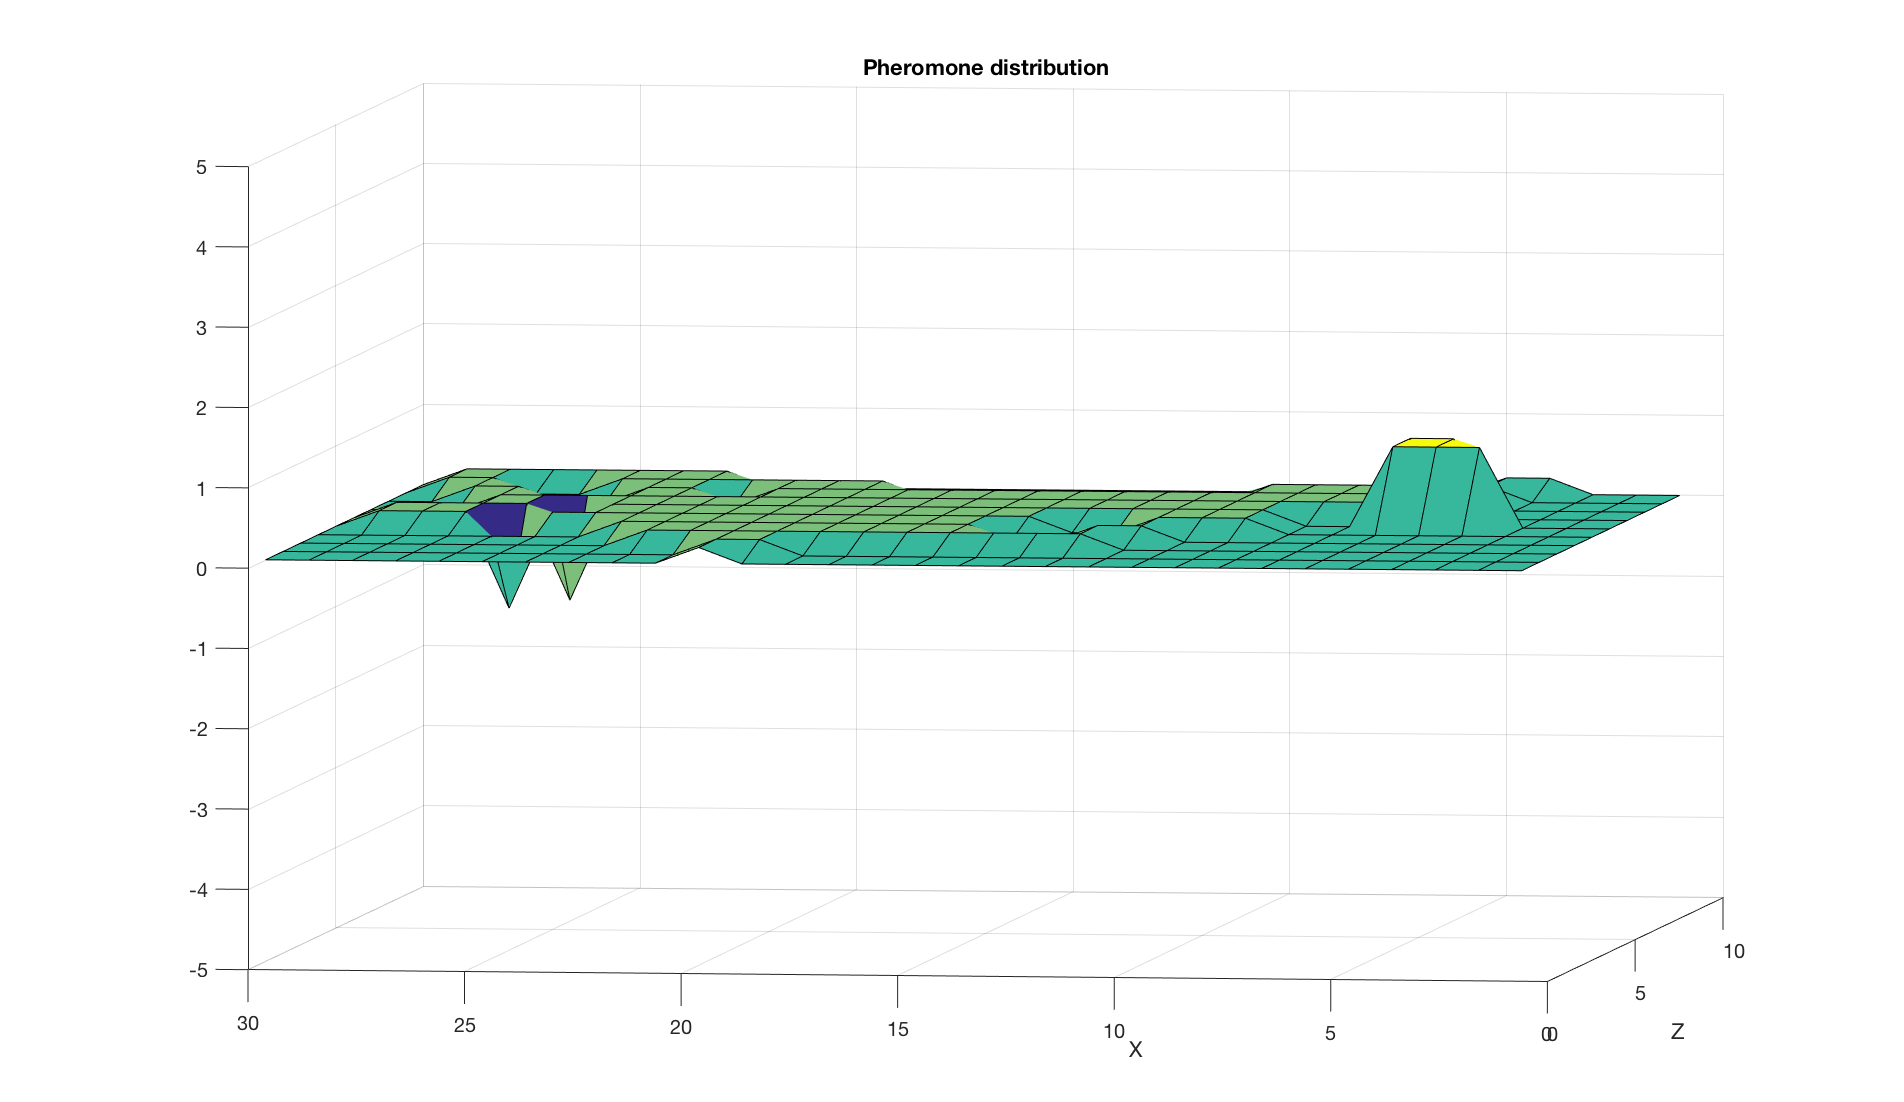
\includegraphics[width=1\columnwidth]{figures/STIG_pheromones}
  	\caption{\label{fig:phero_post}Pheromone grid after simulation has finished (mapped onto the horizontal dimensions)}
\end{figure}


\subsection{Performance}

% Environment Specifications
\begin{table}[H]
\centering
\begin{tabularx}{1\textwidth}{l@{ }Xr}
\toprule
\textbf{Metric} &\textbf{Preference} & \textbf{Kind} \\ \midrule
Number of collisions  & Lowest & $18$  \\
Time spent completing control problem & Lowest & $120.1 seconds$  \\
Utility of space & Lowest & $74\%$  \\
Shape of flight pattern  & N/A & See comments below \\
\bottomrule
\end{tabularx}
\caption{3D Stigmergy performance}
\label{tab:stig_metrics}
\end{table}

\begin{itemize}
\item{\textbf{Number of collisions} - The number of collisions of 18 is acceptable, for a solution spanning 120 seconds. However as Figure \ref{fig:3d_stig_solved} shows, the time spent in collisions is quite high  }
\item{\textbf{Time spend completing the control problem} is twice as high as the shortest path algorithm tested in Section \ref{sec:test_metrics}, however with a lot less collisions.}
\item{\textbf{Utility of space} - This number is ideally balanced with the number of collisions. The utility of space is desired low (which indicates that more agents can be added without causing issues in obstacle avoidance ), as long as it does not create collisions. As the collision number is already 18 over a long period of time, theres no desire to have a lower utility of space in this stigmergy algorithm}
\item{\textbf{Shape of flight pattern} - For this 3D stigmergy algorithm, the flight pattern looks as expected. First the agents search in random locations, before quickly becoming more effective because of the pheromones. The randomness in the flight patterns can be seen in Figure \ref{fig:3d_stig_approx}, where the distances are not constantly minimized, but at multiple times seem to be increasing away from the goal. This happens when the agent does not have a strong enough pheromone follow, in the correct direction. This happens in the beginning, but as the pheromones are developed, the curve becomes steeper downwards, as desired}
\end{itemize}

% Pheromones
\begin{figure}[H]
	\centering
	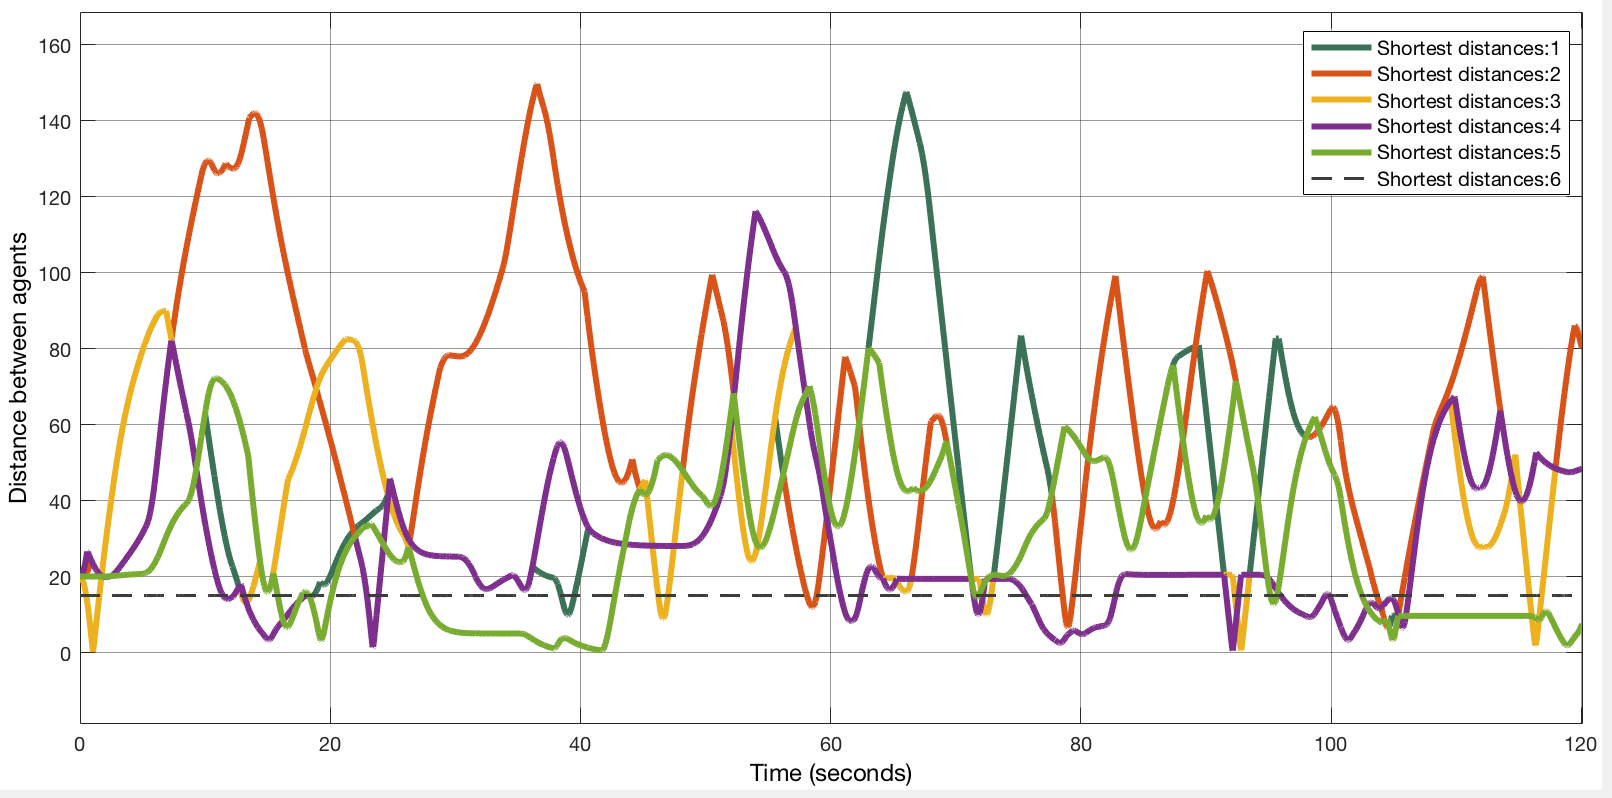
\includegraphics[width=1\columnwidth]{figures/STIG_overlap}
  	\caption{\label{fig:3d_stig_solved}Collisions of agents throughout simulation}
\end{figure}

% Pheromones
\begin{figure}[H]
	\centering
	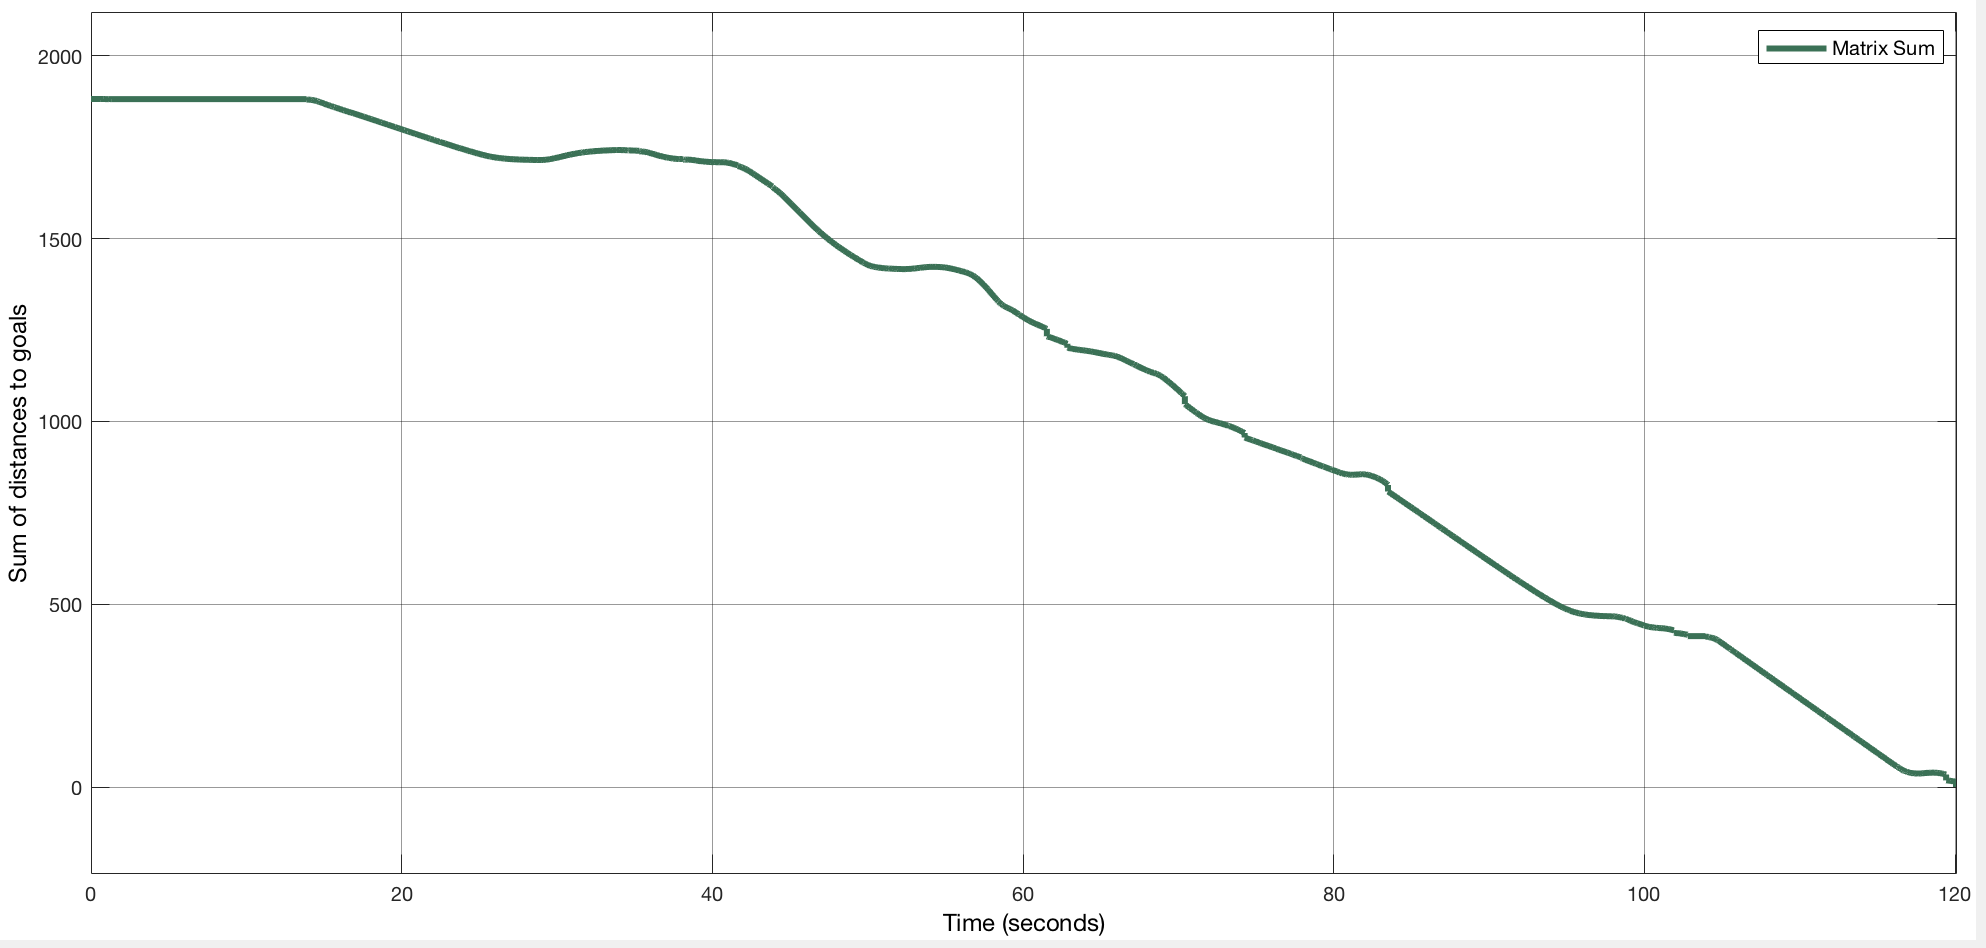
\includegraphics[width=1\columnwidth]{figures/STIG_approx}
  	\caption{\label{fig:3d_stig_approx}Total distances for blocks to goals over time}
\end{figure}

\subsection{Improvement}
The digital pheromones show to be having the desired effects as the curve in Figure \ref{fig:3d_stig_approx}, starts out relatively flat, and then steepens. This shows that the agents are going from moving randomly, to moving according to the pheromones, solving the level faster. 

An area of improvement however is the number of collisions. For this i attempted to implement a layered version of the Stigmergy algorithm of this chapter, which is covered in Chapter \ref{chap:lay_stig}.

  

\chapter{Layered Stigmergy}
\label{chap:lay_stig}


\section{Theory}

\section{Implementation}

\section{Test}
\label{chap:lay_stigmergy.sec:test}  

\chapter{Appendix A}

The following appendix contains the control loop for the non-layered 3-Dimensional Stigmergy implementation. \\

\lstset { %
    language=matlab,
    backgroundcolor=\color{blue!5}, % set backgroundcolor
    basicstyle=\footnotesize,% basic font setting
}

\begin{lstlisting}

for i = 1:length(agents_at)
        
        % Decrease pheromones
        
        index_of_agent = agents_at(i);
        
        % Agent Positions
        agent_x = CX(index_of_agent);
        agent_y = CY(index_of_agent);
        agent_z = CZ(index_of_agent);        
        agent_pos = [agent_x agent_y agent_z];
        
        % Pheromone Index
        p_index_x = floor((agent_x/10)+16);
        p_index_y = floor((agent_y/10)+6);
        p_index_z = floor((agent_z/10)+6);
        
        % Radius limiters when close to envirornment edge
        z_neg = 1;
        z_pos = 1;
        x_neg = 1;
        x_pos = 1;
        
        if p_index_z <= 1 
            p_index_z = 1;
            z_neg = 0;
        elseif p_index_z >= 10 
            p_index_z = 10 ;
            z_pos = 0;
        end
        
        if p_index_y <= 1 
            p_index_y = 1;
        elseif p_index_y >= 10 
            p_index_y = 10 ;
        end
        
        if p_index_x <= 1 
            p_index_x = 1;
            x_neg = 0;
        elseif p_index_x >= 30 
            p_index_x = 30;
            x_pos = 0;
        end
        
        curr_p_index = [p_index_x, p_index_y, p_index_z];
        
        % Value of current pheromone
        % 0: Empty, 1: 
        cur_p_value = pheromones(p_index_x, search_height, p_index_z);
        
       % pheromones(:) = 0;
        % Setting current value to something
        % pheromones(p_index_x, p_index_y, p_index_z) = 0;


        % Assign movement towards box
        if agents_moving_to(i,1) == 0

            % Value, Index of highest element
            [maxval, maxind] = max(pheromones(:));
            [maxxidx, maxyidx, maxzidx] = ind2sub(size(pheromones),maxind);
            
            
            % Agent data
            % 1: State
            % 2,3,4: Coordinates of desired movement
            % 5: Box to carry
            % 6: Pheromoned or random (0:random, 1:p, 2:new p)
            
            if maxval == 0 || agents_moving_to(i, 6) == 2
                agents_moving_to(i, 2) = randi([-149 149],1,1);
                agents_moving_to(i, 3) = search_height; 
                agents_moving_to(i, 4) = randi([-49 49],1,1);
                agents_moving_to(i, 6) = 0;
                
            elseif agents_moving_to(i, 6) == 0;
                disp('Global Pheromone')
                agents_moving_to(i, 6) = 1;
                agents_moving_to(i, 2) = maxxidx*10-150;
                agents_moving_to(i, 3) = search_height; 
                agents_moving_to(i, 4) = maxzidx*10-50;
            else 
                 disp('Local random')
                 agents_moving_to(i, 6) = 2;
                 agents_moving_to(i, 2) = randi([agent_x-20 agent_x+20],1,1);
                 agents_moving_to(i, 3) = search_height; 
                 agents_moving_to(i, 4) = randi([agent_z-20 agent_z+20],1,1);
            end
            
            agents_moving_to(i, 1) = 1;
            
            % Figure
            Y=squeeze(pheromones(:,search_height,:));
            
            x_offset = Y;
            x_offset2 = Y2;

            figure(1), surf(x_offset);
            xlabel('Z'), ylabel('X'), title('Pheromone distribution');
            axis([0 10 0 30 -5 5]);

        elseif agents_moving_to(i,1) == 1
            
            DX(index_of_agent) = agents_moving_to(i, 2);
            DY(index_of_agent) = agents_moving_to(i, 3);
            DZ(index_of_agent) = agents_moving_to(i, 4);
            
            C = [CX(index_of_agent) CY(index_of_agent) CZ(index_of_agent)];

            % Boxes
            box_dist = agent_view_radius;
            closest_box_index = 0;
            for b = 1:last_box_at 
                dist = max(abs([CX(b) CY(b) CZ(b)] - C));
                if blocks_moving_to(b) == 0 && dist <= box_dist
                    box_dist = dist;
                    closest_box_index = b;
                end
            end
           
            if closest_box_index > 0
                DX(index_of_agent) = CX(closest_box_index);
                DY(index_of_agent) = CY(closest_box_index) + block_height;
                DZ(index_of_agent) = CZ(closest_box_index);
            end
                
            D = [DX(index_of_agent) DY(index_of_agent) DZ(index_of_agent)];
            
            % Check if they are standing still, reset
            if max(abs(C-D)) < stand_still_threshold
                if closest_box_index > 0
                    agents_moving_to(i, 1) = 2;
                    blocks_moving_to(closest_box_index) = 1;
                    agents_moving_to(i, 5) = closest_box_index;
                    pheromones(p_index_x, search_height, p_index_z) = 1;  
                elseif agents_moving_to(i, 6) == 0; % if not pheromoned
                    agents_moving_to(i, 1) = 0;
                    disp('Back to search 1');
                else
                    agents_moving_to(i, 1) = 0;
                    disp('Back to search 0');
                end
            elseif cur_p_value == 0;
                pheromones(p_index_x, search_height, p_index_z)  = 0.2; 
            end
            

        % Assign movement towards goal
        elseif agents_moving_to(i,1) == 2
            
            % Value, Index of highest element
            [maxval, maxind] = min(pheromones(:));
            [maxxidx, maxyidx, maxzidx] = ind2sub(size(pheromones),maxind);

            if maxval == 0 || agents_moving_to(i, 6) == 2
                agents_moving_to(i, 2) = randi([-149 149],1,1);
                agents_moving_to(i, 3) = search_height; 
                agents_moving_to(i, 4) = randi([-49 49],1,1);
                agents_moving_to(i, 6) = 0;
                
            elseif agents_moving_to(i, 6) == 0;
                disp('Global Pheromone')
                agents_moving_to(i, 6) = 1;
                agents_moving_to(i, 2) = maxxidx*10-150;
                agents_moving_to(i, 3) = search_height; 
                agents_moving_to(i, 4) = maxzidx*10-50;
            else 
                 disp('Local random')
                 agents_moving_to(i, 6) = 2;
                 agents_moving_to(i, 2) = randi([agent_x-20 agent_x+20],1,1);
                 agents_moving_to(i, 3) = search_height; 
                 agents_moving_to(i, 4) = randi([agent_z-20 agent_z+20],1,1);
            end
            
            agents_moving_to(i, 1) = 3;
            
            % Figure
            Y=squeeze(pheromones(:,search_height,:));
            x_offset = Y;
            figure(1), surf(x_offset);
            xlabel('Z'), ylabel('X'), title('Pheromone distribution');
            axis([0 10 0 30 -5 5])

            
        elseif agents_moving_to(i,1) == 3
            
            index_of_carried = agents_moving_to(i,5);
            
            CX(index_of_carried) = CX(agents_at(i));
            CY(index_of_carried) = CY(agents_at(i))-block_height*.5;
            CZ(index_of_carried) = CZ(agents_at(i));
            
            C = [CX(index_of_agent) CY(index_of_agent) CZ(index_of_agent)];
            
            % Goals
            goal_dist = agent_view_radius;
            closest_goal_index = 0;
            for b = 1:last_box_at 
                dist = max(abs([EX(b) EY(b) EZ(b)] - C));
                if dist <= goal_dist
                    goal_dist = dist;
                    closest_goal_index = b;
                end
            end
            
            % Check if they are standing still, reset
            if closest_goal_index > 0
                DX(index_of_agent) = EX(closest_goal_index);
                DY(index_of_agent) = EY(closest_goal_index)+block_height;
                DZ(index_of_agent) = EZ(closest_goal_index);
            else
                DX(index_of_agent) = agents_moving_to(i, 2);
                DY(index_of_agent) = agents_moving_to(i, 3);
                DZ(index_of_agent) = agents_moving_to(i, 4);
            end
          
            D = [DX(index_of_agent) DY(index_of_agent) DZ(index_of_agent)];
            
            % Check if they are standing still, reset
            if max(abs(C-D)) < stand_still_threshold                
                if closest_goal_index > 0
                    agents_moving_to(i, 1) = 0;
                    agents_moving_to(i, 5) = 0;
                    blocks_moving_to(index_of_carried) = 2;
                    pheromones(p_index_x, search_height, p_index_z)  = - 1;  
                elseif agents_moving_to(i, 6) == 0; % if not pheromoned
                    agents_moving_to(i, 1) = 2;
                    disp('Back to search 3');
                else
                    agents_moving_to(i, 1) = 2;
                    disp('Back to search 4');
                end
            end
            
  
            
        end
    end


\end{lstlisting}  

\chapter{Appendix B}

The following appendix contains the control loop for the layered 3-Dimensional Stigmergy implementation. \\

\lstset { %
    language=matlab,
    backgroundcolor=\color{blue!5}, % set backgroundcolor
    basicstyle=\footnotesize,% basic font setting
}

\begin{lstlisting}


   % Assign Desired Positions
    for i = 1:length(agents_at)
        
        % Decrease pheromones
        
        index_of_agent = agents_at(i);
        
        % Agent Positions
        agent_x = CX(index_of_agent);
        agent_y = CY(index_of_agent);
        agent_z = CZ(index_of_agent);        
        agent_pos = [agent_x agent_y agent_z];
        
        % Pheromone Index
        p_index_x = floor((agent_x/10)+16);
        p_index_y = floor((agent_y/10)+6);
        p_index_z = floor((agent_z/10)+6);
        
        % Radius limiters when close to envirornment edge
        z_neg = 1;
        z_pos = 1;
        x_neg = 1;
        x_pos = 1;
        
        if p_index_z <= 1 
            p_index_z = 1;
            z_neg = 0;
        elseif p_index_z >= 10 
            p_index_z = 10 ;
            z_pos = 0;
        end
        
        if p_index_y <= 1 
            p_index_y = 1;
        elseif p_index_y >= 10 
            p_index_y = 10 ;
        end
        
        if p_index_x <= 1 
            p_index_x = 1;
            x_neg = 0;
        elseif p_index_x >= 30 
            p_index_x = 30;
            x_pos = 0;
        end
        
        curr_p_index = [p_index_x, p_index_y, p_index_z];
        
        % Value of current pheromone
        % 0: Empty, 1: 
        cur_p_value = pheromones(p_index_x, search_height, p_index_z);
        
       % pheromones(:) = 0;
        % Setting current value to something
        % pheromones(p_index_x, p_index_y, p_index_z) = 0;


        % Assign movement towards box
        if agents_moving_to(i,1) == 0

            % Value, Index of highest element
            [maxval, maxind] = max(pheromones(:));
            [maxxidx, maxyidx, maxzidx] = ind2sub(size(pheromones),maxind);
            
            
            % Agent data
            % 1: State
            % 2,3,4: Coordinates of desired movement
            % 5: Box to carry
            % 6: Pheromoned or random (0:random, 1:p, 2:new p)
            
            if maxval == 0 || agents_moving_to(i, 6) == 2
                agents_moving_to(i, 2) = randi([-149 149],1,1);
                agents_moving_to(i, 3) = search_height; 
                agents_moving_to(i, 4) = randi([-49 49],1,1);
                agents_moving_to(i, 6) = 0;
                
            elseif agents_moving_to(i, 6) == 0;
                disp('Global Pheromone')
                agents_moving_to(i, 6) = 1;
                agents_moving_to(i, 2) = maxxidx*10-150;
                agents_moving_to(i, 3) = search_height; 
                agents_moving_to(i, 4) = maxzidx*10-50;
            else 
                 disp('Local random')
                 agents_moving_to(i, 6) = 2;
                 agents_moving_to(i, 2) = randi([agent_x-20 agent_x+20],1,1);
                 agents_moving_to(i, 3) = search_height; 
                 agents_moving_to(i, 4) = randi([agent_z-20 agent_z+20],1,1);
            end
            
            agents_moving_to(i, 1) = 1;
            
            % Figure
            Y=squeeze(pheromones(:,search_height,:));
            Y2=squeeze(pheromone_sources(:,search_height,:));
            
            x_offset = Y;
            x_offset2 = Y2;

            figure(1), surf(x_offset);
            xlabel('Z'), ylabel('X'), title('Pheromone distribution');
            axis([0 10 0 30 -5 5]);
            
            figure(2), surf(x_offset2);
            xlabel('Z'), ylabel('X'), title('Pheromone distribution');
            axis([0 10 0 30 -5 5]);

        elseif agents_moving_to(i,1) == 1
            
            DX(index_of_agent) = agents_moving_to(i, 2);
            DY(index_of_agent) = agents_moving_to(i, 3);
            DZ(index_of_agent) = agents_moving_to(i, 4);
            
            C = [CX(index_of_agent) CY(index_of_agent) CZ(index_of_agent)];

            % Boxes
            box_dist = agent_view_radius;
            closest_box_index = 0;
            for b = 1:last_box_at 
                dist = max(abs([CX(b) CY(b) CZ(b)] - C));
                if blocks_moving_to(b) == 0 && dist <= box_dist
                    box_dist = dist;
                    closest_box_index = b;
                end
            end
           
            if closest_box_index > 0
                DX(index_of_agent) = CX(closest_box_index);
                DY(index_of_agent) = CY(closest_box_index) + block_height;
                DZ(index_of_agent) = CZ(closest_box_index);
            end
                
            D = [DX(index_of_agent) DY(index_of_agent) DZ(index_of_agent)];
            
            % Check if they are standing still, reset
            if max(abs(C-D)) < stand_still_threshold
                if closest_box_index > 0
                    agents_moving_to(i, 1) = 2;
                    blocks_moving_to(closest_box_index) = 1;
                    agents_moving_to(i, 5) = closest_box_index;
                    pheromones(p_index_x, search_height, p_index_z) = 1;  
                elseif agents_moving_to(i, 6) == 0; % if not pheromoned
                    agents_moving_to(i, 1) = 0;
                    disp('Back to search 1');
                else
                    agents_moving_to(i, 1) = 0;
                    disp('Back to search 0');
                end
            elseif cur_p_value == 0;
                pheromones(p_index_x, search_height, p_index_z)  = 0.2; 
            end
          
            % Pheromone sources
            pheromone_sources(p_index_x, search_height, p_index_z) = 0;
            taken = find(pheromone_sources(p_index_x-x_neg:p_index_x+x_pos, 
			search_height, p_index_z-z_neg:p_index_z+z_pos),1);
            pheromone_sources(p_index_x, search_height, p_index_z) = 1;
         
       
            
            pheromone_sources(p_index_x-x_neg:p_index_x+x_pos, 
				search_height, p_index_z-z_neg:p_index_z+z_pos) = 0;
            pheromone_sources(p_index_x, search_height, p_index_z) = 1;
            

            
            

        % Assign movement towards goal
        elseif agents_moving_to(i,1) == 2
            
            % Value, Index of highest element
            [maxval, maxind] = min(pheromones(:));
            [maxxidx, maxyidx, maxzidx] = ind2sub(size(pheromones),maxind);

            if maxval == 0 || agents_moving_to(i, 6) == 2
                agents_moving_to(i, 2) = randi([-149 149],1,1);
                agents_moving_to(i, 3) = search_height; 
                agents_moving_to(i, 4) = randi([-49 49],1,1);
                agents_moving_to(i, 6) = 0;
                
            elseif agents_moving_to(i, 6) == 0;
                disp('Global Pheromone')
                agents_moving_to(i, 6) = 1;
                agents_moving_to(i, 2) = maxxidx*10-150;
                agents_moving_to(i, 3) = search_height; 
                agents_moving_to(i, 4) = maxzidx*10-50;
            else 
                 disp('Local random')
                 agents_moving_to(i, 6) = 2;
                 agents_moving_to(i, 2) = randi([agent_x-20 agent_x+20],1,1);
                 agents_moving_to(i, 3) = search_height; 
                 agents_moving_to(i, 4) = randi([agent_z-20 agent_z+20],1,1);
            end
            
            agents_moving_to(i, 1) = 3;
            
            % Figure
            Y=squeeze(pheromones(:,search_height,:));
            x_offset = Y;
            figure(1), surf(x_offset);
            xlabel('Z'), ylabel('X'), title('Pheromone distribution');
            axis([0 10 0 30 -5 5])

            
        elseif agents_moving_to(i,1) == 3
            
            index_of_carried = agents_moving_to(i,5);
            
            CX(index_of_carried) = CX(agents_at(i));
            CY(index_of_carried) = CY(agents_at(i))-block_height*.5;
            CZ(index_of_carried) = CZ(agents_at(i));
            
            C = [CX(index_of_agent) CY(index_of_agent) CZ(index_of_agent)];
            
            % Goals
            goal_dist = agent_view_radius;
            closest_goal_index = 0;
            for b = 1:last_box_at 
                dist = max(abs([EX(b) EY(b) EZ(b)] - C));
                if dist <= goal_dist
                    goal_dist = dist;
                    closest_goal_index = b;
                end
            end
            
            % Check if they are standing still, reset
            if closest_goal_index > 0
                DX(index_of_agent) = EX(closest_goal_index);
                DY(index_of_agent) = EY(closest_goal_index)+block_height;
                DZ(index_of_agent) = EZ(closest_goal_index);
            else
                DX(index_of_agent) = agents_moving_to(i, 2);
                DY(index_of_agent) = agents_moving_to(i, 3);
                DZ(index_of_agent) = agents_moving_to(i, 4);
            end
          
            D = [DX(index_of_agent) DY(index_of_agent) DZ(index_of_agent)];
            
            % Check if they are standing still, reset
            if max(abs(C-D)) < stand_still_threshold                
                if closest_goal_index > 0
                    agents_moving_to(i, 1) = 0;
                    agents_moving_to(i, 5) = 0;
                    blocks_moving_to(index_of_carried) = 2;
                    pheromones(p_index_x, search_height, p_index_z)  = - 1;  
                elseif agents_moving_to(i, 6) == 0; % if not pheromoned
                    agents_moving_to(i, 1) = 2;
                    disp('Back to search 3');
                else
                    agents_moving_to(i, 1) = 2;
                    disp('Back to search 4');
                end
            end
            
            
            % Sources of pheromones
            pheromone_sources(p_index_x-x_neg:p_index_x+x_pos, 
		search_height, p_index_z-z_neg:p_index_z+z_pos) = 0;
            pheromone_sources(p_index_x, search_height, p_index_z) = 1;
            
        end
    end

\end{lstlisting}  



%\include{Chapter2}                                 		%Chapter 2
\appendix
                              %Appendix A

%-----------
% Backmatter
%-----------
%\backmatter
\nocite{*}                        
\renewcommand{\sectionmark}[1]{\markright{#1}}
\sectionmark{Bibliography}
\addcontentsline{toc}{chapter}{Bibliography}        %Force addition of Bibliography to TOC
\bibliographystyle{alpha}                           %Use alpha codes for references
\bibliography{References}  
\end{document}
% % % EOF % % %